\section{Scheduling}

Scheduling is the problem of deciding which process/thread on every core in the system is currently executing. This decision must be dynamically, not static. First we need to introduce some terminology. Notice how the wait time is defined as the combination of hold time and execution time.
\begin{center}
	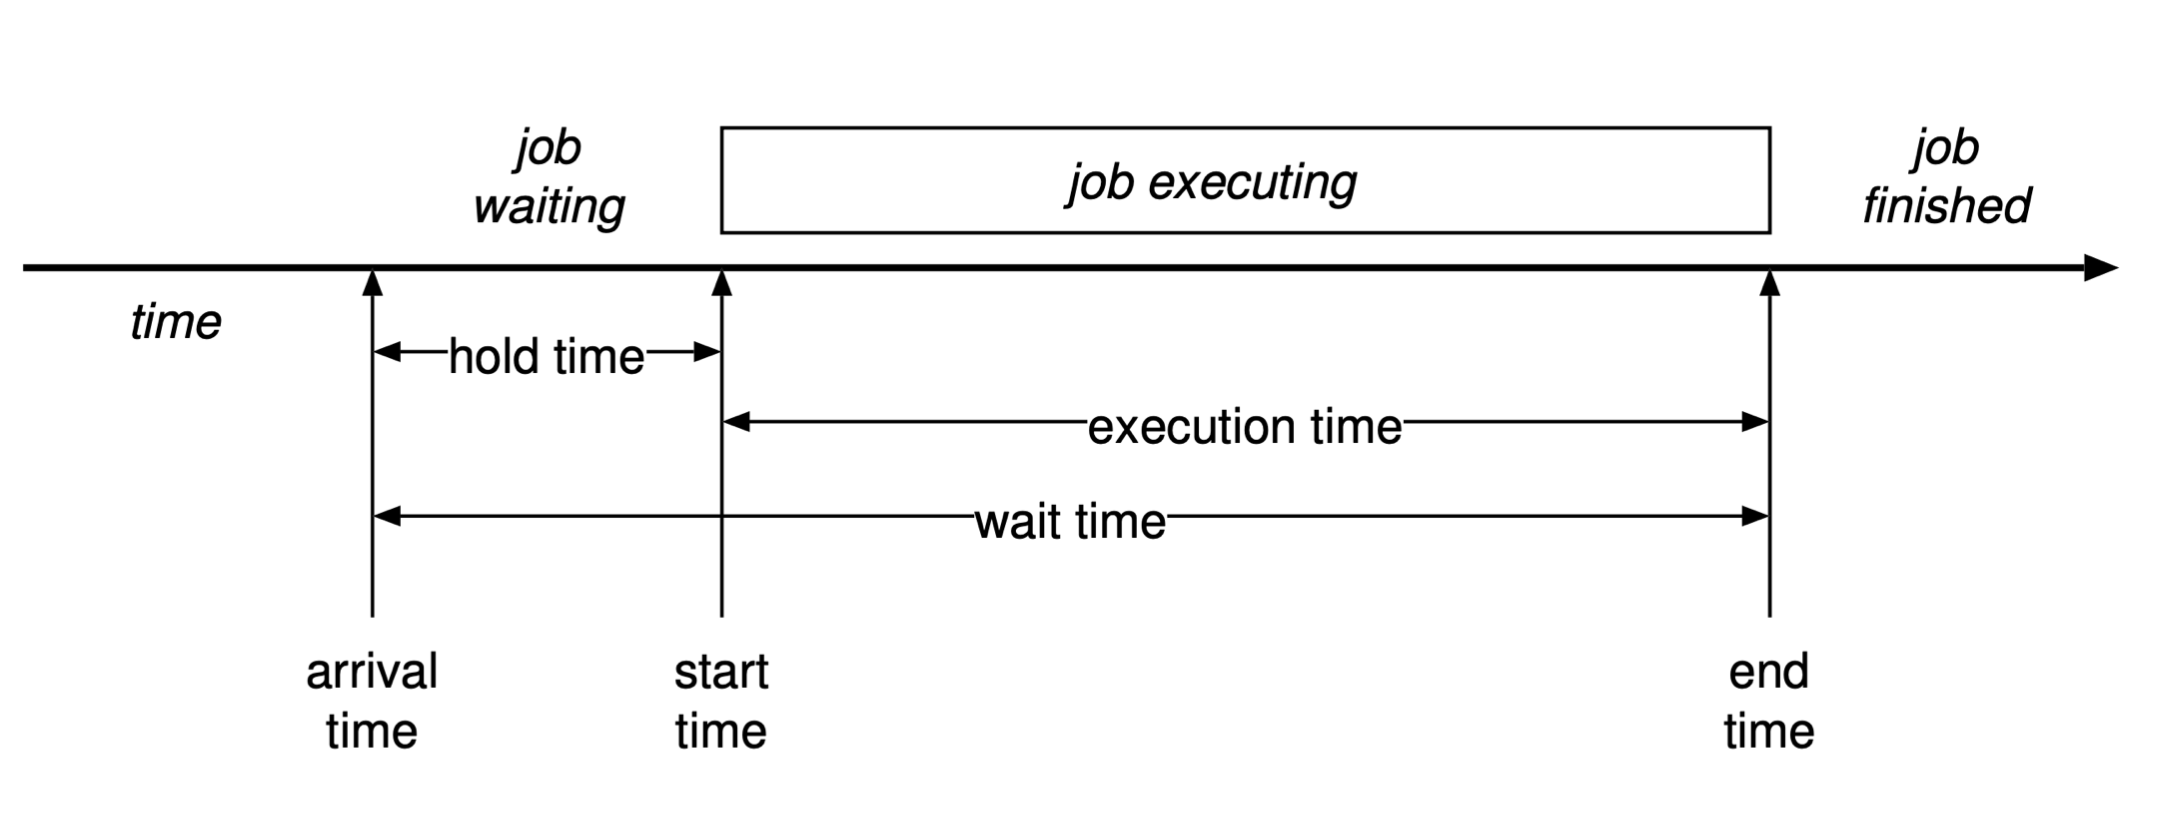
\includegraphics[width=\linewidth]{scheduling.png}
\end{center}

The important metrics for scheduling are throughput (rate of completing jobs) and overhead (time spent without a job executing). \medskip

In the following part we will look at various scheduling algorithms, starting from a very simple approach.


\subsection{Non-Preemptive Batch Oriented}

There are two basic algorithms:
\begin{itemize}
	\item First Come First Served
	\item Shortest Job First
\end{itemize}

Both are algorithms are very simple to implement but their applications are limited.


\subsection{Preemptive Batch Oriented}

We introduce preemption, meaning that we interrupt the execution after some finite time interval. After such an interrupt we decide which program to run next. \medskip

\textbf{Modified SJF:} Go through the sorted list of jobs and execute each until interrupted. Note that the length of a job does not get recomputed after an execution.


\subsection{Interactive Scheduling}

When running interactive workload, we can encounter events that block the execution (I/O, page-faults, etc.). During this time we would like to run another program instead of wasting execution time. \medskip

\textbf{Round Robin Scheduling:} Let $R$ be a queue and $q$ be the scheduling quantum:
\begin{enumerate}
	\item Set an interval timer for an interrupt $q$ seconds in the future
	\item Dispatch the job at the head of $R$
	\item If blocking happens or the timer runs out, return to the scheduler
	\item Push the previously running job to the tail of $R$
\end{enumerate}

\textbf{Priority Based Scheduling:} We assign a priority to each task and dispatch the highest priority task first, if we have ties we use RR to break them. To avoid starvation we might want to use dynamic priorities (increased priority depending on wait time). An even more complex approach is to introduce multi-level queues, meaning that we have a fixed number of queues that assign priorities within each queue. Then we use RR scheduling between the queues to execute tasks. \medskip

Priority scheduling runs into problems when a high priority process has to wait for a lock from a low priority process (Priority Inversion). To fix this, we can either introduce inheritance - the holder of the lock acquires the priority of the highest waiting process - or ceiling - the holder of the lock runs at the highest priority.


\subsection{Linux o(1) Scheduler}

Linux uses 140 multilevel feedback queues, each with a different priority. Multilevel feedback queues penalize CPU bound tasks and prioritize I/O operations, as I/O tasks will eventually block. \medskip

The priority range 0-99 is used for high priority, static tasks and it uses FCFS or RR scheduling. The range 100-139 is for user tasks and uses RR together with priority ageing for I/O tasks.
